\documentclass[11pt]{article}
\usepackage[utf8]{inputenc}
\usepackage[dvips]{graphicx}
\usepackage{fancybox}
\usepackage{verbatim}
\usepackage{array}
\usepackage{latexsym}
\usepackage{alltt}
\usepackage{hyperref}
\usepackage{textcomp}
\usepackage{color}
\usepackage{amsmath}
\usepackage{amsfonts}
\usepackage{tikz}
\usepackage{fitch}  % to use fitch
\usepackage{float}
\usepackage[hmargin=3cm,vmargin=5.0cm]{geometry}
%\topmargin=0cm
\topmargin=-2cm
\addtolength{\textheight}{6.5cm}
\addtolength{\textwidth}{2.0cm}
%\setlength{\leftmargin}{-5cm}
\setlength{\oddsidemargin}{0.0cm}
\setlength{\evensidemargin}{0.0cm}


\begin{document}

\section*{Student Information } 
Full Name : Anıl Eren Göçer\\
Id Number : 2448397 \\

\section*{Answer 1}

\section*{a)}
$L_0 = [(a \cup b)^*aa(a \cup b)^*bb(a \cup b)^*] \space \space \space \cup \space \space \space [(a \cup b)^*bb(a \cup b)^*aa(a \cup b)^*]$

\section*{b)}


\begin{center}
\begin{tikzpicture}[scale=0.2]
\tikzstyle{every node}+=[inner sep=0pt]
\draw [black] (5.9,-27.8) circle (3);
\draw (5.9,-27.8) node {$q_0$};
\draw [black] (13.6,-14.8) circle (3);
\draw (13.6,-14.8) node {$q_1$};
\draw [black] (29.7,-14.8) circle (3);
\draw (29.7,-14.8) node {$q_2$};
\draw [black] (44,-14.8) circle (3);
\draw (44,-14.8) node {$q_3$};
\draw [black] (59.9,-14.8) circle (3);
\draw (59.9,-14.8) node {$q_4$};
\draw [black] (73.6,-27.8) circle (3);
\draw (73.6,-27.8) node {$q_9$};
\draw [black] (28.9,-41.5) circle (3);
\draw (28.9,-41.5) node {$q_6$};
\draw [black] (44,-41.5) circle (3);
\draw (44,-41.5) node {$q_7$};
\draw [black] (59.9,-41.5) circle (3);
\draw (59.9,-41.5) node {$q_8$};
\draw [black] (13.6,-41.5) circle (3);
\draw (13.6,-41.5) node {$q_5$};
\draw [black] (7.43,-25.22) -- (12.07,-17.38);
\fill [black] (12.07,-17.38) -- (11.23,-17.81) -- (12.09,-18.32);
\draw (10.4,-22.55) node [right] {$e$};
\draw [black] (12.277,-12.12) arc (234:-54:2.25);
\draw (13.6,-7.55) node [above] {$a,b$};
\fill [black] (14.92,-12.12) -- (15.8,-11.77) -- (14.99,-11.18);
\draw [black] (16.6,-14.8) -- (26.7,-14.8);
\fill [black] (26.7,-14.8) -- (25.9,-14.3) -- (25.9,-15.3);
\draw (21.65,-15.3) node [below] {$a$};
\draw [black] (40.8,-14.8) -- (41,-14.8);
\fill [black] (41,-14.8) -- (40.2,-14.3) -- (40.2,-15.3);
\draw [black] (7.6,-30.4) -- (12.17,-38.86);
\fill [black] (12.17,-38.86) -- (12.23,-37.92) -- (11.35,-38.39);
\draw [black] (72.277,-25.12) arc (234:-54:2.25);
\draw (73.6,-20.55) node [above] {$a,b$};
\fill [black] (74.92,-25.12) -- (75.8,-24.77) -- (74.99,-24.18);
\draw [black] (42.677,-12.12) arc (234:-54:2.25);
\draw (44,-7.55) node [above] {$a,b$};
\fill [black] (45.32,-12.12) -- (46.2,-11.77) -- (45.39,-11.18);
\draw [black] (45.323,-44.18) arc (54:-234:2.25);
\draw (44,-48.75) node [below] {$a,b$};
\fill [black] (42.68,-44.18) -- (41.8,-44.53) -- (42.61,-45.12);
\draw [black] (14.923,-44.18) arc (54:-234:2.25);
\draw (13.6,-48.75) node [below] {$a,b$};
\fill [black] (12.28,-44.18) -- (11.4,-44.53) -- (12.21,-45.12);
\draw [black] (16.6,-41.5) -- (25.9,-41.5);
\fill [black] (25.9,-41.5) -- (25.1,-41) -- (25.1,-42);
\draw (21.25,-42) node [below] {$b$};
\draw [black] (31.9,-41.5) -- (41,-41.5);
\fill [black] (41,-41.5) -- (40.2,-41) -- (40.2,-42);
\draw (36.45,-42) node [below] {$b$};
\draw [black] (47,-41.5) -- (56.9,-41.5);
\fill [black] (56.9,-41.5) -- (56.1,-41) -- (56.1,-42);
\draw (51.95,-42) node [below] {$a$};
\draw [black] (62.02,-39.38) -- (71.48,-29.92);
\fill [black] (71.48,-29.92) -- (70.56,-30.13) -- (71.27,-30.84);
\draw (67.72,-35.13) node [below] {$a$};
\draw [black] (32.7,-14.8) -- (41,-14.8);
\fill [black] (41,-14.8) -- (40.2,-14.3) -- (40.2,-15.3);
\draw (36.85,-15.3) node [below] {$a$};
\draw [black] (47,-14.8) -- (56.9,-14.8);
\fill [black] (56.9,-14.8) -- (56.1,-14.3) -- (56.1,-15.3);
\draw (51.95,-15.3) node [below] {$b$};
\draw [black] (62.08,-16.86) -- (71.42,-25.74);
\fill [black] (71.42,-25.74) -- (71.19,-24.82) -- (70.5,-25.55);
\draw (65.73,-21.78) node [below] {$b$};
\draw [black] (0.5,-27.8) -- (2.9,-27.8);
\fill [black] (2.9,-27.8) -- (2.1,-27.3) -- (2.1,-28.3);
\end{tikzpicture}
\end{center}

\begin{center}
    M: The NFA recognizing the language $L_0$
\end{center} 

\noindent Now, let's formally define M:  \\ \\
M = (K,$\Sigma$,$\delta$,s,F) where , \\ \\
K = $\{q_0,q_1,q_2,q_3,q_4,q_5,q_6,q_7,q_8,q_9\}$ \\
$\Sigma$ = $\{a,b\}$ \\
s = $q_0$ \\ \\
F = \{$q_9$\} \\ \\
and, \\ \\

\noindent $\delta$ = $\{(q_0,\epsilon,q_1), (q_0,\epsilon,q_5), (q_1,a,q_1), (q_1,b,q_1), (q_1,a,q_2) (q_2,a,q_3), (q_3,a,q_3), (q_3,b,q_3), (q_3,b,q_4), (q_4,b,q_9),\\ (q_5,a,q_5), (q_5,b,q_5), (q_5,b,q_6), (q_6,b,q_7), (q_7,a,q_7), (q_7,b,q_7), (q_7,a,q_8), (q_8,a,q_9), (q_9,a,q_9),(q_9,b,q_9)\}$.  \newpage



\section*{c)}
Let's construct a DFA, called $M^'$ = $(K^'$, $ \Sigma$ , $ \delta^'$, $ s^'$, $ F^'$), which is equivalent to the NFA in part b. \\

\noindent Let's apply the subset construction algorithm to M. Since M has 10 states, $M^'$ will have $2^{10}$ states. However, only few of these states will be relevant to the operation of $M^'$ i.e. those states that can be reached from state $s^'$ by reading some input string. Obviously, any state in $K^'$ that is not reachable from $s^'$ is irrelevant to
the operation of $M^'$ and to the language accepted by it. We shall build this reachable part of $M^'$ by starting from
$s^'$ and introducing a new state only when it is needed as the value of $\delta^{'}(q,x)$ for some state $q \in K^'$ already introduced and some $x \in \Sigma$.  \\ 

\noindent Now, let's define $\epsilon$-closure of each state in M. \\

\noindent $E$($q_0$) = $\{q_0,q_1,q_5\}$ \indent \indent E($q_5$) = $\{q_5\}$ \\
\noindent $E$($q_1$) = $\{q_1\}$ \indent \indent \indent \space \space \space  $E$($q_6$) = $\{q_6\}$

\noindent $E$($q_2$) = $\{q_2\}$ \indent \indent \indent \space \space \space  $E$($q_7$) = $\{q_7\}$ \\
\noindent $E$($q_3$) = $\{q_3\}$ \indent \indent \indent \space \space \space  $E$($q_8$) = $\{q_8\}$ \\
\noindent $E$($q_4$) = $\{q_4\}$ \indent \indent \indent \space \space \space  $E$($q_9$) = $\{q_9\}$ \\ \\ 

\noindent Since $s^'$ = E($q_0$) = $\{q_0,q_1,q_5\}$ \\

\noindent $(q_1,a,q_1)$, $(q_1,a,q_2)$, $(q_5,a,q_6)$ are all transition of the form (q,a,p) for some q \in $ s^'$. It follows that \\

$\delta^{'}(s^{'},a)$ = $E(q_1) \cup E(q_2) \cup E(q_5) = \{q1,q2,q5\}$ \\

\noindent $(q_1,b,q_1)$, $(q_5,b,q_5)$, $(q_5,b,q_6)$ are all transition of the form (q,b,p) for some q \in $ s^'$. \\

$\delta^{'}(s^{'},b)$ = $E(q_1) \cup E(q_5) \cup E(q_6) = \{q1,q5,q6\}$ \\ \\

\noindent \textbf{Repeating this calculation for the newly introduced states}, we have the following: \\ 

$\delta^{'}(\{q_1,q_2,q_5\},a) = \{q_1,q_2,q_3,q_5\}$  \\
\indent $\delta^{'}(\{q_1,q_2,q_5\},b) = \{q_1,q_5,q_6\}$ \\ 

$\delta^{'}(\{q_1,q_5,q_6\},a) = \{q_1,q_2,q_5\}$  \\
\indent $\delta^{'}(\{q_1,q_5,q_6\},b) = \{q_1,q_5,q_6,q_7\}$  \\

$\delta^{'}(\{q_1,q_2,q_3,q_5\},a) = \{q_1,q_2,q_3,q_5\}$  \\
\indent $\delta^{'}(\{q_1,q_2,q_3,q_5\},b) = \{q_1,q_3,q_4,q_5,q_6\}$  \\

$\delta^{'}(\{q_1,q_5,q_6,q_7\},a) = \{q_1,q_2,q_5,q_7,q_8\}$  \\
\indent $\delta^{'}(\{q_1,q_5,q_6,q_7\},b) = \{q_1,q_5,q_6,q_7\}$  \\

$\delta^{'}(\{q_1,q_3,q_4,q_5,q_6\},a) = \{q_1,q_2,q_3,q_5\}$  \\
\indent $\delta^{'}(\{q_1,q_3,q_4,q_5,q_6\},b) = \{q_1,q_3,q_4,q_5,q_6,q_7,q_9\}$  \\ \newpage

$\delta^{'}(\{q_1,q_2,q_5,q_7,q_8\},a) = \{q_1,q_2,q_3,q_5,q_7,q_8,q_9\}$  \\
\indent $\delta^{'}(\{q_1,q_2,q_5,q_7,q_8\},b) = \{q_1,q_5,q_6,q_7\}$  \\

$\delta^{'}(\{q_1,q_3,q_4,q_5,q_6,q_7,q_9\},a) = \{q_1,q_2,q_3,q_5,q_7,q_8,q_9\}$  \\
\indent $\delta^{'}(\{q_1,q_3,q_4,q_5,q_6,q_7,q_9\},a) = \{q_1,q_3,q_4,q_5,q_6,q_7,q_9\}$ \\

$\delta^{'}(\{q_1,q_2,q_3,q_5,q_7,q_8,q_9\},a) = \{q_1,q_2,q_3,q_5,q_7,q_8,q_9\}$  \\
\indent $\delta^{'}(\{q_1,q_2,q_3,q_5,q_7,q_8,q_9\},b) = \{q_1,q_3,q_4,q_5,q_6,q_7,q_9\}$  \\ \\

\noindent $F^'$, the set of final states, contains each set of states of which $q_9$ is a member, since $q_9$ is the sole member of F. So,  $\{q_1,q_3,q_4,q_5,q_6,q_7,q_9\}$, $\{q_1,q_2,q_3,q_5,q_7,q_8,q_9\}$ are final states. \\

\begin{center}
    State Diagram of the $M^'$
\end{center}
\begin{center}
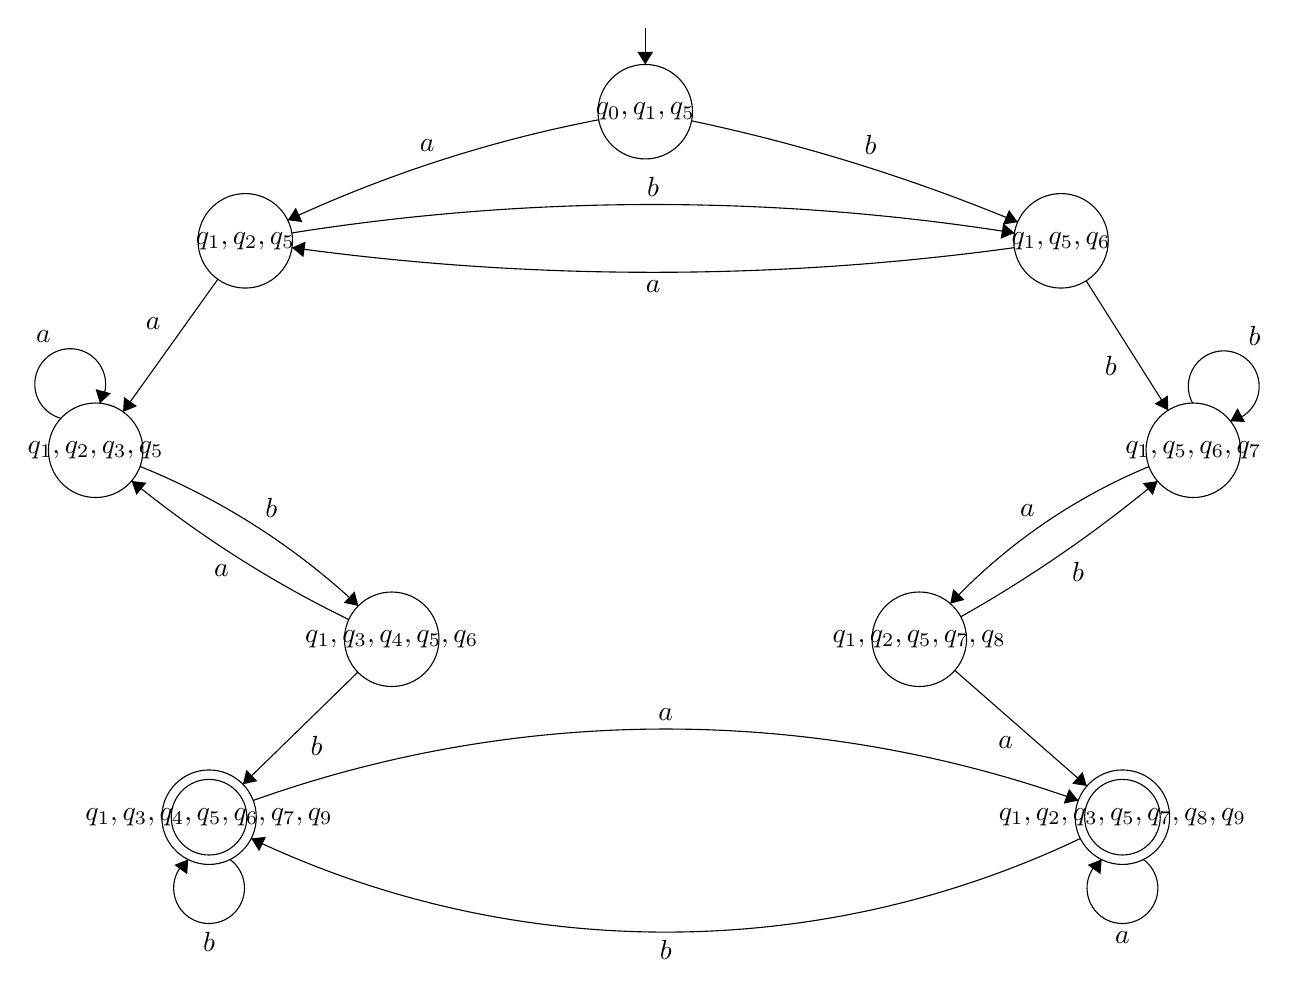
\begin{tikzpicture}[scale=0.2]
\tikzstyle{every node}+=[inner sep=0pt]
\draw [black] (39.9,-4.9) circle (3);
\draw (39.9,-4.9) node {${q_0,q_1,q_5}$};
\draw [black] (14.5,-13.1) circle (3);
\draw (14.5,-13.1) node {${q_1,q_2,q_5}$};
\draw [black] (66.3,-13.1) circle (3);
\draw (66.3,-13.1) node {${q_1,q_5,q_6}$};
\draw [black] (5,-26.4) circle (3);
\draw (5,-26.4) node {${q_1,q_2,q_3,q_5}$};
\draw [black] (74.7,-26.4) circle (3);
\draw (74.7,-26.4) node {${q_1,q_5,q_6,q_7}$};
\draw [black] (23.8,-38.4) circle (3);
\draw (23.8,-38.4) node {${q_1,q_3,q_4,q_5,q_6}$};
\draw [black] (57.3,-38.4) circle (3);
\draw (57.3,-38.4) node {${q_1,q_2,q_5,q_7,q_8}$};
\draw [black] (12.2,-49.7) circle (3);
\draw (12.2,-49.7) node {${q_1,q_3,q_4,q_5,q_6,q_7,q_9}$};
\draw [black] (12.2,-49.7) circle (2.4);
\draw [black] (70.2,-49.7) circle (3);
\draw (70.2,-49.7) node {${q_1,q_2,q_3,q_5,q_7,q_8,q_9}$};
\draw [black] (70.2,-49.7) circle (2.4);
\draw [black] (39.9,0.4) -- (39.9,-1.9);
\fill [black] (39.9,-1.9) -- (40.4,-1.1) -- (39.4,-1.1);
\draw [black] (17.198,-11.789) arc (114.90099:100.88276:85.021);
\fill [black] (17.2,-11.79) -- (18.13,-11.91) -- (17.71,-11);
\draw (26.05,-7.46) node [above] {$a$};
\draw [black] (42.843,-5.481) arc (78.08831:67.40147:116.392);
\fill [black] (63.55,-11.91) -- (63,-11.14) -- (62.61,-12.07);
\draw (54.2,-7.67) node [above] {$b$};
\draw [black] (12.76,-15.54) -- (6.74,-23.96);
\fill [black] (6.74,-23.96) -- (7.62,-23.6) -- (6.8,-23.02);
\draw (9.16,-18.38) node [left] {$a$};
\draw [black] (17.458,-12.6) arc (99.00985:80.99015:146.497);
\fill [black] (63.34,-12.6) -- (62.63,-11.98) -- (62.47,-12.97);
\draw (40.4,-10.29) node [above] {$b$};
\draw [black] (63.332,-13.534) arc (-82.18579:-97.81421:168.663);
\fill [black] (17.47,-13.53) -- (18.19,-14.14) -- (18.33,-13.15);
\draw (40.4,-15.6) node [below] {$a$};
\draw [black] (67.9,-15.64) -- (73.1,-23.86);
\fill [black] (73.1,-23.86) -- (73.09,-22.92) -- (72.25,-23.45);
\draw (69.87,-21.05) node [left] {$b$};
\draw [black] (2.804,-24.374) arc (255.03751:-32.96249:2.25);
\draw (1.69,-19.58) node [above] {$a$};
\fill [black] (5.27,-23.42) -- (5.96,-22.78) -- (5,-22.52);
\draw [black] (74.658,-23.412) arc (208.53189:-79.46811:2.25);
\draw (78.59,-19.8) node [above] {$b$};
\fill [black] (77.05,-24.55) -- (77.99,-24.61) -- (77.51,-23.73);
\draw [black] (7.818,-27.427) arc (68.05043:46.84956:44.704);
\fill [black] (21.68,-36.28) -- (21.44,-35.36) -- (20.76,-36.09);
\draw (16.16,-30.71) node [above] {$b$};
\draw [black] (21.074,-37.148) arc (-115.88999:-129.21001:70.533);
\fill [black] (7.28,-28.35) -- (7.59,-29.24) -- (8.22,-28.46);
\draw (12.98,-33.65) node [below] {$a$};
\draw [black] (59.268,-36.137) arc (136.65478:112.5298:36.671);
\fill [black] (59.27,-36.14) -- (60.18,-35.9) -- (59.45,-35.21);
\draw (64.17,-30.62) node [above] {$a$};
\draw [black] (72.428,-28.359) arc (-50.25087:-60.56456:84.398);
\fill [black] (72.43,-28.36) -- (71.49,-28.49) -- (72.13,-29.25);
\draw (67.38,-33.45) node [below] {$b$};
\draw [black] (21.65,-40.49) -- (14.35,-47.61);
\fill [black] (14.35,-47.61) -- (15.27,-47.41) -- (14.57,-46.69);
\draw (19.02,-44.53) node [below] {$b$};
\draw [black] (59.56,-40.38) -- (67.94,-47.72);
\fill [black] (67.94,-47.72) -- (67.67,-46.82) -- (67.01,-47.57);
\draw (62.79,-44.54) node [below] {$a$};
\draw [black] (13.523,-52.38) arc (54:-234:2.25);
\draw (12.2,-56.95) node [below] {$b$};
\fill [black] (10.88,-52.38) -- (10,-52.73) -- (10.81,-53.32);
\draw [black] (71.523,-52.38) arc (54:-234:2.25);
\draw (70.2,-56.95) node [below] {$a$};
\fill [black] (68.88,-52.38) -- (68,-52.73) -- (68.81,-53.32);
\draw [black] (15.005,-48.637) arc (109.65473:70.34527:77.88);
\fill [black] (67.39,-48.64) -- (66.81,-47.9) -- (66.47,-48.84);
\draw (41.2,-43.6) node [above] {$a$};
\draw [black] (67.524,-51.055) arc (-64.55437:-115.44563:61.267);
\fill [black] (14.88,-51.05) -- (15.38,-51.85) -- (15.81,-50.95);
\draw (41.2,-57.5) node [below] {$b$};
\end{tikzpicture}
\end{center}

\newpage

\section*{d)}

\textbf{Trace on NFA: } \\

\noindent $w'$ is accepted if and only if there is at least one sequence of moves terminating at a final state. \\

\noindent There are 8 possible sequence of moves which this NFA can follow when it is given $w'$. We need to check all of them. \\

\textbf{1)}  
$(q_0,bbabb) $ \vdash $ (q_1,bbabb)$ \vdash $ (q_1,babb)$ \vdash $ (q_1,abb)$ \vdash $ (q_1,bb)$ \vdash $ (q_1,b)$ \vdash $ (q_1,\epsilon)$ \\ \\
\indent The NFA terminates at $q_1$, which is not a final state. \\ \\

\textbf{2)} $(q_0,bbabb) $ \vdash $ (q_1,bbabb) $ \vdash $ (q_1,babb) $ \vdash $ (q_1,abb) $ \vdash $ (q_2,bb)$ \\ \\
\indent The NFA gets stuck at $q_2$. \\ \\

\textbf{3)} $(q_0,bbabb) $ \vdash $ (q_5,bbabb) $ \vdash $ (q_5,babb) $ \vdash $ (q_5,abb) $ \vdash $ (q_5,bb) $ \vdash $ (q_5,b) $ \vdash $ (q_5,\epsilon)$ \\ \\
\indent The NFA terminates at $q_5$, which is not a final state. \\ \\

\textbf{4)} $(q_0,bbabb) $ \vdash $ (q_5,bbabb) $ \vdash $ (q_5,babb) $ \vdash $ (q_5,abb) $ \vdash $ (q_5,bb) $ \vdash $ (q_5,b) $ \vdash $ (q_6,\epsilon)$ \\ \\
\indent The NFA terminates at $q_6$, which is not a final state. \\ \\

\textbf{5)} $(q_0,bbabb) $ \vdash $ (q_5,bbabb) $ \vdash $ (q_5,babb) $ \vdash $ (q_5,abb) $ \vdash $ (q_5,bb) $ \vdash $ (q_6,b) $ \vdash $ (q_7,\epsilon)$ \\ \\
\indent The NFA terminates at $q_7$, which is not a final state. \\ \\

\textbf{2)} $(q_0,bbabb) $ \vdash $ (q_5,bbabb) $ \vdash $ (q_5,babb) $ \vdash $ (q_6,abb) $ \vdash $ (q_2,bb)$ \\ \\
\indent The NFA gets stuck at $q_6$. \\ \\

\textbf{7)} $(q_0,bbabb) $ \vdash $ (q_5,bbabb) $ \vdash $ (q_6,babb) $ \vdash $ (q_7,abb) $ \vdash $ (q_7,bb) $ \vdash $ (q_7,b) $ \vdash $ (q_7,\epsilon)$ \\ \\
\indent The NFA terminates at $q_7$, which is not a final state. \\ \\

\textbf{8)} $(q_0,bbabb) $ \vdash $ (q_5,bbabb) $ \vdash $ (q_6,babb) $ \vdash $ (q_7,abb) $ \vdash $ (q_8,bb)$ \\ \\
\indent The NFA gets stuck at $q_8$. \\ \\

\noindent Therefore, there is no sequence of moves terminating at a final state. Hence, $w^'$ is \textbf{not accepted} by the NFA. \newpage

\noindent \textbf{Trace on DFA:} \\ \\

$(\{q_0,q_1,q_5\},bbabb)$ \vdash $(\{q_1,q_5,q_5\},babb)$ \\
\indent \indent \indent \indent \indent \indent \space \space \vdash $(\{q_1,q_5,q_6,q_7\},abb)$ \\ 
\indent \indent \indent \indent \indent \indent \space \space  \vdash $(\{q_1,q_2,q_5,q_7,
q_8\},bb)$ \\
\indent \indent \indent \indent \indent \indent \space \space  \vdash $(\{q_1,q_5,q_6,q_7\},b)$ \\
\indent \indent \indent \indent \indent \indent \space \space  \vdash $(\{q_1,q_5,q_6,q_7\},\epsilon)$ \\

\noindent As you can see, the DFA terminates at the state $(\{q_1,q_5,q_6,q_7\}$, which is not a final (accept) state. Hence, $w^'$ is \textbf{not accepted} by the DFA.












\newpage

\section*{Answer 2}

\section*{a)} \\
Assume that $L_{1}$ is regular. \\ \\
\indent Let $p$ be the \textbf{pumping length} for $L_{1}$ given by the pumping lemma. \\ \\

Let s = $a^{p+1}b^{p}$. Then s can be split into s = xyz, satisfying the conditions of the pumping lemma which are as follows: \\

(1) For each i \geq 0, $ xy^{i}z $ \in $ L_{1}$. \\
\indent (2) $|y|$ $>$ 0 \\
\indent (3) $|xy|$ \leq p \\ \\

By condition 3 of the pumping lemma, $|xy| \leq p$, y consists only of a's. \\ \\

The pumping lemma states that $ xy^{i}z $ \in $ L_{1}$ even when i = 0, so let's consider string $xy^{0}z = xz$ . \\ Removing string y decreases the number of a's in s because of condition 2 of pumping lemma, $|y| > 0$. Recall that s has just one more a than b. Therefore,
xz cannot have more a's than b's, so it cannot be a member of $L_1$. Thus, we obtain a contradiction.  \\ \\

\noindent
Hence, $L_1$ is not regular. \\ \\

\noindent Remember that class of regular languages is closed under complementation. So, a language A is
regular if and only if $\overline{A}$ is regular.  This means that class of non-regular languages is also closed under complementation, so a languages A is non-regular if and only if
$\overline{A}$ is non regular. \\ \\

\noindent As seen abover, we have proven that $L_1$ is non-regular. Thus, $\overline{L_1}$ is also non-regular. \\ \\

\noindent Hence, $L_2 = L_1$ is \textbf{not regular} . 









\newpage
\section*{b)} \\
Note that $L_4$ is a subset of $L_5$, namely $L_4 \subseteq L_5$. \\

\noindent Thus, $L_4 \cup L_5 \equiv L_5$  \\

\noindent Observe that $L_5 = \{\epsilon, a, b, aa, bb, ab, ......\}$ = $a^*b^*$. \\ \\

\noindent Also, $L_5$ is recognized by the finite automaton given below:  \\ \\

\begin{center}
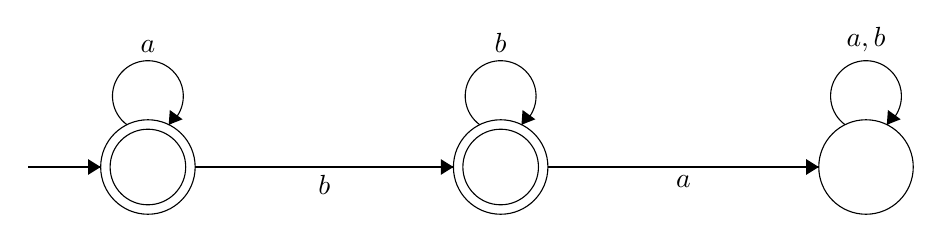
\begin{tikzpicture}[scale=0.2]
\tikzstyle{every node}+=[inner sep=0pt]
\draw [black] (17.5,-30.3) circle (3);
\draw [black] (17.5,-30.3) circle (2.4);
\draw [black] (39.9,-30.3) circle (3);
\draw [black] (39.9,-30.3) circle (2.4);
\draw [black] (63.1,-30.3) circle (3);
\draw [black] (9.9,-30.3) -- (14.5,-30.3);
\fill [black] (14.5,-30.3) -- (13.7,-29.8) -- (13.7,-30.8);
\draw [black] (16.177,-27.62) arc (234:-54:2.25);
\draw (17.5,-23.05) node [above] {$a$};
\fill [black] (18.82,-27.62) -- (19.7,-27.27) -- (18.89,-26.68);
\draw [black] (20.5,-30.3) -- (36.9,-30.3);
\fill [black] (36.9,-30.3) -- (36.1,-29.8) -- (36.1,-30.8);
\draw (28.7,-30.8) node [below] {$b$};
\draw [black] (38.577,-27.62) arc (234:-54:2.25);
\draw (39.9,-23.05) node [above] {$b$};
\fill [black] (41.22,-27.62) -- (42.1,-27.27) -- (41.29,-26.68);
\draw [black] (42.9,-30.3) -- (60.1,-30.3);
\fill [black] (60.1,-30.3) -- (59.3,-29.8) -- (59.3,-30.8);
\draw (51.5,-30.8) node [below] {$a$};
\draw [black] (61.777,-27.62) arc (234:-54:2.25);
\draw (63.1,-23.05) node [above] {$a,b$};
\fill [black] (64.42,-27.62) -- (65.3,-27.27) -- (64.49,-26.68);
\end{tikzpicture}
\end{center} 

\\
\noindent Thus, $L_5$ is regular.  \\ \\

\noindent Now, consider $L_6 = b^*a(ab^*a)^*$. Because $L_6$ is generated by a regular expression, $L_6$ is regular.   \\ \\

\noindent Note that $L_4 \cup L_5 \cup L_6 \equiv L_5 \cup L_6$ . \\ \\

\noindent We have shown that $L_5$ and $L_6$ are regular. \\ \\

\noindent Since regular languages are closed under union. $L_5 \cup L_6$ is regular. \\ \\ \\

\noindent Thus, $L_4 \cup L_5 \cup L_6$ is \textbf{regular} .



\end{document}
